\documentclass[a4paper]{article}
\usepackage{minted}

\usepackage{polski}
\usepackage[utf8]{inputenc}

\usepackage[export]{adjustbox}
\usepackage{scrextend}
\usepackage{amsfonts}
\usepackage{amsmath}


\usepackage{geometry}
\geometry{a4paper, left=15mm, top=30mm, right=15mm, bottom=20mm}

\usepackage{gensymb}
\usepackage{graphicx} 
\usepackage{isotope}
\usepackage{array}
\usepackage{float}
\usepackage{titlesec}
\usepackage{fancyhdr}
\usepackage{multirow}

\usepackage{hyperref}
\usepackage{sectsty}
\usepackage{enumitem}
\usepackage{listings}
\usepackage[labelformat=simple]{subcaption}
\usepackage{xcolor,colortbl}


\usepackage{tikz}
\usetikzlibrary{shapes.geometric, arrows}
\tikzstyle{startstop} = [
    rectangle, 
    rounded corners, 
    minimum width=3cm, minimum height=1cm,
    text centered,
    draw=black, fill=red!30]
\tikzstyle{io} = [
    trapezium, trapezium left angle=70, trapezium right angle=110, 
    minimum width=3cm, minimum height=1cm, 
    text centered, 
    draw=black, fill=blue!30]
\tikzstyle{process} = [
    rectangle, 
    minimum width=3cm, minimum height=1cm, 
    text centered, 
    draw=black, fill=orange!30]
\tikzstyle{decision} = [
    diamond, 
    minimum width=3cm, minimum height=1cm, 
    text centered, 
    draw=black, fill=green!30]
\tikzstyle{arrow} = [thick,->,>=stealth]

\usepackage{karnaugh-map}

\sectionfont{\normalfont\huge\sectionrule{0pt}{0pt}{-6pt}{1pt}}
\subsectionfont{\normalfont\LARGE}
\subsubsectionfont{\normalfont\Large}

\pagestyle{fancy}
\fancyhf{}
\fancyhead[LE,LO]{\Large Łukasz Kwinta, Kacper Kozubowski, Ida Ciepiela}
\fancyhead[LE,RO]{\Large Układ FPGA}
\fancyfoot[CE,CO]{\Large\thepage}

\renewcommand{\footrulewidth}{1pt}
\renewcommand{\headrulewidth}{1pt}

\definecolor{Gray}{gray}{0.85}
\definecolor{LightGray}{gray}{0.95}

\newcolumntype{a}{>{\columncolor{Gray}}c}
\newcolumntype{b}{>{\columncolor{white}}c}

\hypersetup{
    colorlinks,
    citecolor=black,
    filecolor=black,
    linkcolor=black,
    urlcolor=black
}

\counterwithin{table}{section}
\counterwithin{figure}{section}

\title{\fontsize{30pt}{30pt}\selectfont Laboratorium 4 \\ Układ FPGA}
\author{\fontsize{20pt}{20pt}\selectfont Łukasz Kwinta, Kacper Kozubowski, Ida Ciepiela}
\date{maj 2024}

\begin{document}
\maketitle
\pagebreak
\large
\tableofcontents

\pagebreak
\section{Cel zadania}
\Large
Celem laboratorium było zaprogramowanie układu FPGA tak aby wyświetlał animację poruszających się 
segmentów na obrzeżach wyświetlaczy 7 segmentowych. Należało również, zaimplementować prostą funkcjonalność 
obejmującą zmianę prędkości i kierunku ruchu świetlnego odcinka, przy pomocy znajdujących się na płytce przycisków.  

\section{Czym są układy FPGA?}
FPGA (Field-Programmable Gate Array) to rodzaj układu logicznego,
który można programować po jego wyprodukowaniu. W przeciwieństwie do tradycyjnych układów ASIC (Application-Specific Integrated Circuit), 
które są zaprojektowane do wykonywania jednego konkretnego zadania i nie mogą być zmieniane po wyprodukowaniu, 
FPGA oferują elastyczność i możliwość wielokrotnego programowania. 
Kluczowym aspektem takiego układu jest matryca programowalnych bloków logicznych i konfigurowalnych połączeń.

Bloki logiczne to podstawowe jednostki wykonujące logikę i arytmetykę.
Każdy blok zawiera programowalne elementy, takie jak bramki logiczne,
multiplexery, oraz przerzutniki, które można konfigurować do wykonywania różnych funkcji.
Natomiast, sieć połączeń umożliwia łączenie tych bloków w dowolny sposób.

Dzięki takiej konstrukcji układy FPGA można dostosować do różnych zastosowań, 
co czyni je niezwykle wszechstronnymi w inżynierii cyfrowej.

\begin{figure}[H]
    \centering
    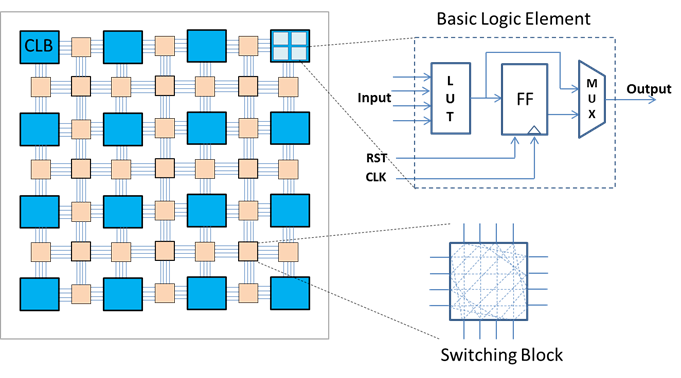
\includegraphics[width=0.75\textwidth]{FPGA_diagram.png}
    \caption{Przykładowy schemat układu FPGA}
\end{figure}

\pagebreak
\section{Realizacja}
Do napisania programu na układ FPGA, spełniającego warunki zadania, wykorzystaliśmy język opisu sprzętu Verilog, a także
oprogramowanie Vivado ML Edition od firmy Xilinx.
Dostarczone przez nas rozwiązanie zostało przygotowane na płytkę Nexys-A7 50T.

\begin{figure}[H]
    \centering
    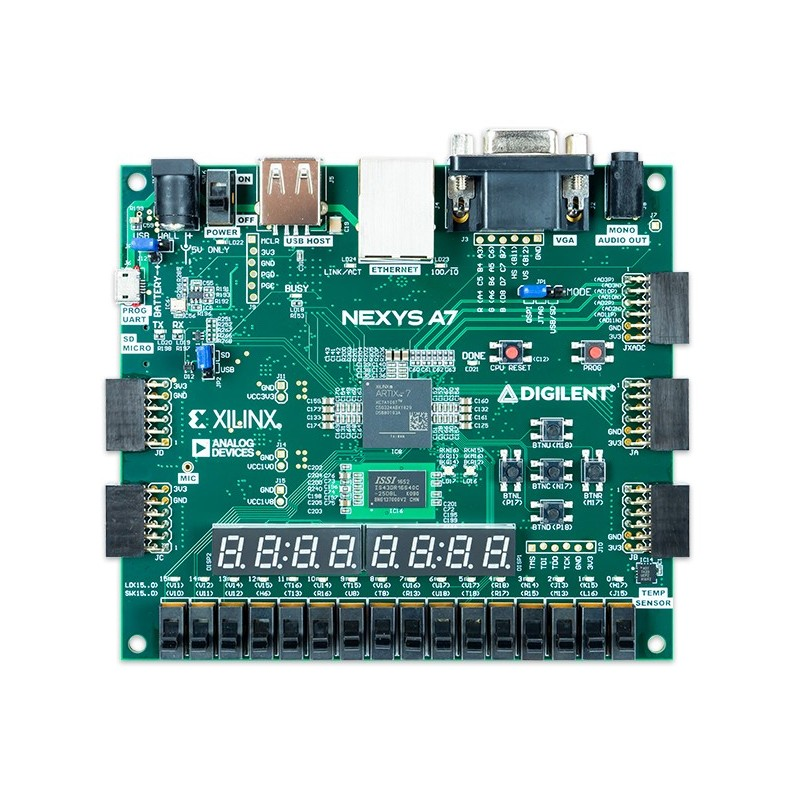
\includegraphics[width=\textwidth]{nexys-a7-artix-50t-fpga-xilinx-edu.jpg}
    \caption{Wykorzystana płytka z układem FPGA}
\end{figure}

\section{Rozwiązanie}
\begin{figure}[H]
    \centering
    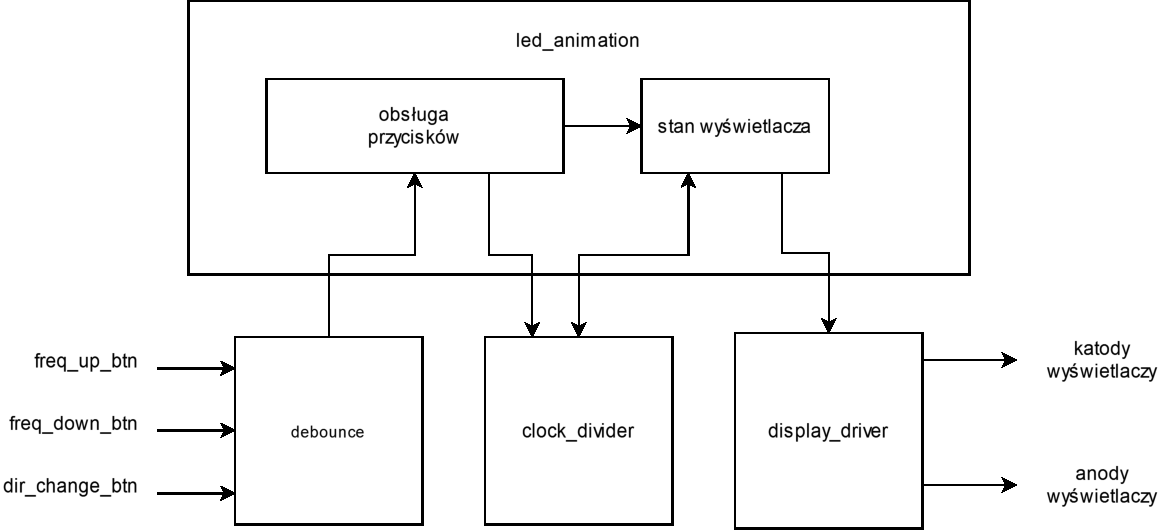
\includegraphics[width=\textwidth]{led_animation.drawio.pdf}
    \caption{Schemat blokowy rozwiązania}
\end{figure}
\subsection{Moduł dzielnika częstotliwości}
Aby w łatwy sposób zmieniać prędkość animacji, zdecydowaliśmy się na zastosowanie modułu dzielnika częstotliwości.
Moduł przyjmuje na wejściu zegar systemowy oraz rejestr oznaczający obecny okres
zegara wyjściowego. Następnie zlicza on takty zegara systemowego i gdy licznik dojdzie
do zadanej wartości, zmienia stan zegara wyjściowego na przeciwny.
\begin{minted}[
    frame=lines,
    framesep=2mm,
    baselinestretch=1.2,
    bgcolor=LightGray,
    fontsize=\footnotesize,
    linenos
]{verilog}
// moduł dzielący zegar
module clock_divider(
    input integer clock_period,
    input wire clk,
    
    output reg divided_clock
);


initial
    divided_clock <= 0;

longint counter_value = 0;

// zliczamy zadany okres zegara (ilość cykli zegara wejściowego), i gdy 
// doliczymy do konca zmieniamy stan spowolnionego zegara na przeciwny
always@ (posedge clk)
begin 
    if (counter_value >= clock_period) 
        begin
            divided_clock <= ~divided_clock;
            counter_value <= 0;
        end
    else 
        begin
            divided_clock <= divided_clock;
            counter_value <= counter_value + 1;
        end
end

endmodule
\end{minted}
\subsection{Moduł filtrujący przyciski}
Aby uniknąć efektu drgania styków przycisków, zdecydowaliśmy się na zastosowanie modułu
filtrującego wejście przycisków. Działa on na bardzo prostej zasadzie - zlicza on ilość 
cykli zegara systemowego w których przycisk jest w stanie wysokim - wciśnięty. Gdy ilość
cykli przekroczy zadaną wartość, przycisk uznawany jest za wciśnięty. Każdy stan niski 
pomiędzy kolejnymi resetuje licznik. Długość odliczania można ustawić poprzez
parametr DEBOUNCE\_TIME przy instancjonowaniu modułu.
\begin{minted}[
    frame=lines,
    framesep=2mm,
    baselinestretch=1.2,
    bgcolor=LightGray,
    fontsize=\footnotesize,
    linenos
]{verilog}
// moduł filtrujący przyciski
module debounce #(parameter DEBOUNCE_TIME = 1000 * 100) (
    input wire clk,
    input wire button_physical,
    
    output reg button_active
);

// ustawiamy początkowy stan przycisku na 0
initial
    button_active = 0;

integer btn_clock_cycles_counter = 0;

// zliczamy zadaną ilość cykli zegara 
// jeśli w którymś cyklu przycisk będzie w stanie niskimi,
// resetujemy licznik wartości
always@ (posedge clk)
begin
   if (button_physical == 1)
       begin
            btn_clock_cycles_counter <= btn_clock_cycles_counter + 1;
            if (btn_clock_cycles_counter >= DEBOUNCE_TIME) 
                button_active <= 1;
       end
    else 
        begin
            btn_clock_cycles_counter <= 0;
            button_active <= 0;
        end
        
end

endmodule
\end{minted}
\pagebreak
\subsection{Moduł sterujący wyświetlaczami}
Aby wyświetlać wiele segmentów wielu wyświetlaczach 7 segmentowych na raz,
musieliśmy zaimplementować moduł sterujący wyświetlaczami. Moduł ten 
odświeża wyświetlacze z zadaną częstotliwością po kolei, tak aby 
stworzyć wrażenie, że wiele wyświetlaczy aktywnych jest w jednym czasie.

\begin{figure}[H]
    \centering
    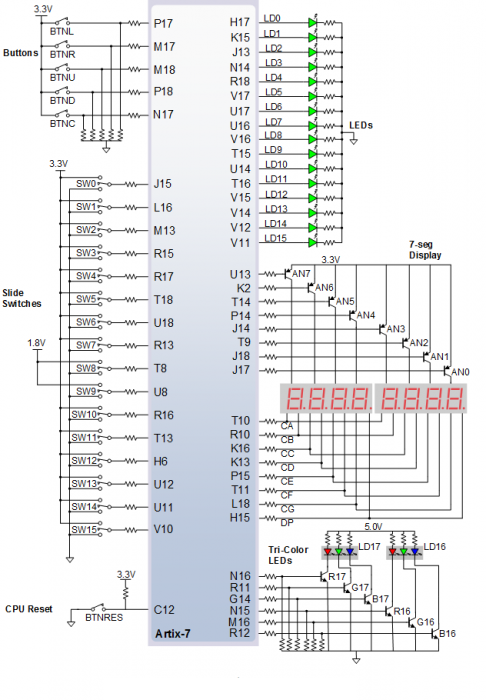
\includegraphics[width=0.6\textwidth]{fpga_led_diagram.png}
    \caption{Schemat podpięcia wyświetlaczy do układu FPGA}
\end{figure}

Zabieg ten musieliśmy zastosować gdyż wszystkie wyświetlacze 
mają wspólne katody segmentów co oznacza, że przy aktywacji 
anody wielu wyświetlaczy w jednym czasie, będą one wyświetlać te same 
segmenty.

\begin{minted}[
    frame=lines,
    framesep=2mm,
    baselinestretch=1.2,
    bgcolor=LightGray,
    fontsize=\footnotesize,
    linenos
]{verilog}
module displays_driver #(parameter REFERESH_PERIOD = 100 * 1000)(
    input wire clk,
    
    // rejestr wejściowy określający stan wszystkich wyświetlaczy
    input reg [7:0] display [7:0],
    
    // wyjscia steujace wyswietlaczami
    // stan niski na danym indeksie aktywuje dany wyswietlacz
    output reg [7:0] sseg_anodes,
    
    // |   7   |   6   |   5   |   4   |   3   |   2   |   1   |   0   |
    // |  DP   |   CG  |  CF   |  CE   |  CD   |  CC   |  CB   |  CA   |
    // stan niski na danym indeksie aktywuje dany segment na wszystkich aktywnych wyswietlaczach
    output reg [7:0] sseg_cathodes
);

initial 
begin
    sseg_anodes <= '1;
    sseg_cathodes <= '1;
end

reg refresh_clk; //1 khz refresh clock
clock_divider clk_div (
    .clock_period(REFERESH_PERIOD),
    .clk(clk),
    .divided_clock(refresh_clk)
);

reg [3:0] display_number = 0;

always@ (posedge refresh_clk)
begin 
    sseg_anodes = '1;
    sseg_anodes[display_number] <= 0;
    sseg_cathodes <= 8'(~display[display_number]);
    
    display_number = display_number + 1;
    if (display_number >= `DISPLAY_COUNT)
        display_number <= 0;
end

endmodule
\end{minted}

\subsection{Właściwy moduł generujący animację}
Główny moduł całego programu. Definiuje użyteczne makra, obsługuje wszystkie inne moduły
przekazując im odpowiednie argumenty,
przyjmuje i obsługuje sygnały wejściowe z przycisków oraz kontroluje
wyświetlanie animacji.
Dzięki odpowiednio zaimplementowanej logice możliwe jest wywołanie animacji na dowolnej liczbie liniowo ułożonych 
wyświetlaczy, po zmianie jednego parametru. 


\begin{minted}[
    frame=lines,
    framesep=2mm,
    baselinestretch=1.2,
    bgcolor=LightGray,
    fontsize=\footnotesize,
    linenos
]{verilog}
`timescale 1ns / 1ps // tylko dla symulacji

// Przydatne makra dla wyswietlaczow
`define SEGMENT_A_MASK 8'(1 << 0)
`define SEGMENT_B_MASK 8'(1 << 1)
`define SEGMENT_C_MASK 8'(1 << 2)
`define SEGMENT_D_MASK 8'(1 << 3)
`define SEGMENT_E_MASK 8'(1 << 4)
`define SEGMENT_F_MASK 8'(1 << 5)
`define SEGMENT_G_MASK 8'(1 << 6)
`define SEGMENT_DOT_MASK 8'(1 << 7)
`define DISPLAY_CLEAR '0
`define DISPLAY_ALL '1

`define DISPLAY_REFRESH_FREQUENCY (100 * 1000 / 8) // częstotliwość odświeżania ekranów = 0,125kHz
`define START_ANIMATION_PERIOD (1000*100*1000 / 4) // okres startowy = 0,25s
`define MAX_ANIMATION_PERIOD 1000*100*1000*100 // maks okres = 100s
`define MIN_ANIMATION_PERIOD 1

`define DISPLAY_COUNT 8 // liczba wykorzystywanych wyświetlaczy

`define MAX_SNAKE_LENGTH (`DISPLAY_COUNT*2 + 3)
`define START_SNAKE_LENGTH 1
`define MIN_SNAKE_LENGTH 1


/* Definicja modułu z wejsciami i wyjsciami zdefiniowanymi w pliku .xdc */
module led_animation(
    // wejscia przycisków
    input wire btn_freq_up,
    input wire btn_freq_dn,
    input wire btn_dir,
    input wire len_up,
    input wire len_dn,
    
    input wire clk, // zegar systemowy 100Mhz
    
    // wyjscia steujace wyswietlaczami
    // stan niski na danym indeksie aktywuje dany wyswietlacz
    output reg [7:0] sseg_anodes,
    
    // |   7   |   6   |   5   |   4   |   3   |   2   |   1   |   0   |
    // |  DP   |   CG  |  CF   |  CE   |  CD   |  CC   |  CB   |  CA   |
    // stan niski na danym indeksie aktywuje dany segment na wszystkich aktywnych wyswietlaczach
    output reg [7:0] sseg_cathodes,
    
    // wyjscie sterujace ledem
    output wire clk_led
);

initial
begin
    sseg_cathodes <= '1;
    sseg_anodes <= '1;
end

// startowy okres spowolnionego zegara
longint clock_period = `START_ANIMATION_PERIOD;

// użycie modułu spowalniającego zegar
reg divided_clk;
assign clk_led = divided_clk;
clock_divider clk_div (
    .clock_period(clock_period),
    .clk(clk),
    .divided_clock(divided_clk)
);

reg [7:0] display [7:0];
displays_driver display_driver (
    .clk(clk),
    .display(display),
    .sseg_anodes(sseg_anodes),
    .sseg_cathodes(sseg_cathodes)
);
defparam display_driver.REFERESH_PERIOD = `DISPLAY_REFRESH_FREQUENCY;

// definicja kierunku poruszania sie segmentu
enum {LEFT, RIGHT} dir = RIGHT;

localparam num_of_segments = (4 + `DISPLAY_COUNT * 2);
integer curr_state = 0;
integer curr_display = 0;

// robimy cykliczną kolejkę do przechowywania informacji o zaświeconych segmentach
integer snake[0:num_of_segments][0:1]; 
integer head = `START_SNAKE_LENGTH - 1;
integer tail = 0;

integer length = `START_SNAKE_LENGTH;
integer old_length = `START_SNAKE_LENGTH;

integer i; 
initial begin
    for (i = 0; i < num_of_segments; i = i + 1)
        begin
            snake[i][0] = -1;
            snake[i][1] = 0;
        end 
    for (i = 0; i < `DISPLAY_COUNT; i = i + 1)
        display[i] = `DISPLAY_CLEAR;
end

// przejście na kolejny segment
always@ (posedge divided_clk)
begin
    if (dir == RIGHT)
        curr_state = (curr_state + 1);
    else
        curr_state = (curr_state - 1);
        
    if (curr_state < 0)
        curr_state = num_of_segments + curr_state;
        
    else if (curr_state > num_of_segments - 1)
        curr_state = curr_state - num_of_segments;
end

always@ (posedge divided_clk)
begin
    if (old_length > length) 
        begin
            display[snake[tail][0]] = display[snake[tail][0]] - 2**(snake[tail][1]);
            
            tail = tail + 1;
            old_length = old_length - 1;
            if (tail == num_of_segments)
                tail = 0;
            display[snake[tail][0]] = display[snake[tail][0]] - 2**(snake[tail][1]);
        end
    else if (old_length < length) 
        begin
            tail = tail - 1;
            old_length = old_length + 1;
            if (tail < 0)
                tail = num_of_segments - 1;
        end
        
    else if (snake[tail][0] != -1) // gasimy ogon
        begin
            display[snake[tail][0]] = display[snake[tail][0]] - 2**(snake[tail][1]);
        end
        
    // uaktualnienie wskaźników
    tail = tail + 1;
    head = head + 1;
    if (head == num_of_segments)
        head = 0;
    if (tail == num_of_segments)
        tail = 0;
    
    snake[head][0] = curr_display;

    if (curr_display == 0) // obsługa prawego wyświetlacza
        begin           
            snake[head][1] = curr_state;
            display[0] = display[0] + 2**curr_state;
            
            if ((dir == LEFT && curr_state == 0) || (dir == RIGHT && curr_state == 3))
                curr_display = curr_display + 1;
        end
    
    else if (curr_display == (`DISPLAY_COUNT - 1)) // obsługa lewego wyświetlacza
        begin
            snake[head][1] = (curr_state - (`DISPLAY_COUNT - 1) < 6 ? curr_state - (`DISPLAY_COUNT - 1) : 0);
            display[`DISPLAY_COUNT - 1] = display[`DISPLAY_COUNT - 1] + 2**(curr_state - (`DISPLAY_COUNT - 1) < 6 
                                                                            ? curr_state - (`DISPLAY_COUNT - 1) : 0);
            
            if ((dir == LEFT && curr_state == (`DISPLAY_COUNT + 2)) 
                 || (dir == RIGHT && curr_state == (`DISPLAY_COUNT + 5)))
                curr_display = curr_display - 1;
        end
                
    else if (curr_state > 3 && curr_state < (`DISPLAY_COUNT + 2)) // obsługa dolnych segmentów
        begin
            snake[head][1] = 3;
            display[curr_display] = display[curr_display] + 2**3;
            
            if (dir == RIGHT)
                curr_display = (curr_display + 1) & (`DISPLAY_COUNT - 1);
            
            else
                curr_display = (curr_display - 1) & (`DISPLAY_COUNT - 1);
        end
    else // obsługa górnych segmentów
        begin
            snake[head][1] = 0;
            display[curr_display] = display[curr_display] + 2**0;
            
            if (dir == RIGHT)
                curr_display = (curr_display - 1) & (`DISPLAY_COUNT - 1);

            else
                curr_display = (curr_display + 1) & (`DISPLAY_COUNT - 1);
        end
end



// użycie modułu filtrującego zakłócenia przycisków
reg button_dir_active, button_freq_up_active, button_freq_dn_active, button_len_dn_active, button_len_up_active;
debounce dir_debounce ( 
    .clk(clk),
    .button_physical(btn_dir),
    .button_active(button_dir_active)
);

debounce freq_up_debounce ( 
    .clk(clk),
    .button_physical(btn_freq_up),
    .button_active(button_freq_up_active)
);

debounce freq_dn_debounce ( 
    .clk(clk),
    .button_physical(btn_freq_dn),
    .button_active(button_freq_dn_active)
);

debounce len_dn_debounce ( 
    .clk(clk),
    .button_physical(len_dn),
    .button_active(button_len_dn_active)
);

debounce len_up_debounce ( 
    .clk(clk),
    .button_physical(len_up),
    .button_active(button_len_up_active)
);

reg button_freq_up_old = 0;
reg button_freq_dn_old = 0;
reg button_dir_old = 0;
reg button_len_up_old = 0;
reg button_len_dn_old = 0;

reg button_freq_up_raise = 0;
reg button_freq_dn_raise = 0;
reg button_dir_raise = 0;
reg button_len_up_raise = 0;
reg button_len_dn_raise = 0;

// blok wykrywający narastające stanu przyciku poprzez porównanie starej wartosci z nową wartością
always@ (posedge clk)
begin
    if (button_freq_up_active != button_freq_up_old && button_freq_up_active == 1)
        button_freq_up_raise <= 1;
        
    if (button_freq_dn_active != button_freq_dn_old && button_freq_dn_active == 1)
        button_freq_dn_raise <= 1;
        
    if (button_dir_active != button_dir_old && button_dir_active == 1)
        button_dir_raise <= 1;
        
    if (button_len_up_active != button_len_up_old && button_len_up_active == 1)
        button_len_up_raise <= 1;
        
    if (button_len_dn_active != button_len_dn_old && button_len_dn_active == 1)
        button_len_dn_raise <= 1;
       
    if (button_freq_up_raise == 1)
        if (clock_period > `MIN_ANIMATION_PERIOD)
            clock_period <= clock_period >> 1;
       
    if (button_freq_dn_raise == 1)
        if (clock_period < `MAX_ANIMATION_PERIOD) 
            clock_period <= clock_period << 1;
        
    if (button_dir_raise == 1)
        if(dir == LEFT) dir <= RIGHT;
        else            dir <= LEFT;
    
    if (button_len_up_raise == 1)
        if (length < `MAX_SNAKE_LENGTH) 
            length <= length + 1;
            
    if (button_len_dn_raise == 1)
        if (length > `MIN_SNAKE_LENGTH) 
             length <= length - 1;
        
    button_freq_dn_old <= button_freq_dn_active;
    button_freq_up_old <= button_freq_up_active;
    button_dir_old <= button_dir_active;
    button_len_up_old <= button_len_up_active;
    button_len_dn_old <= button_len_dn_active;
        
    button_freq_up_raise = 0;
    button_freq_dn_raise = 0;
    button_dir_raise = 0;
    button_len_up_raise = 0;
    button_len_dn_raise = 0;
end

endmodule
\end{minted}

\pagebreak
\section{Zastosowania układów FPGA}
Układy FPGA znajdują szerokie zastosowanie w wielu dziedzinach,
dzięki swojej elastyczności, wydajności i możliwości szybkiej rekonfiguracji.
Poniżej przedstawiamy kilka przykładów:

\begin{itemize}
    \item Są wykorzystywane w routerach, switchach i bramkach sieciowych do szybkiego przetwarzania pakietów danych.
    \item Wykorzystywane są w urządzeniach audio, sprzęcie muzycznym, systemach obróbki obrazu oraz w systemach medycznych, takich jak USG czy MRI
    \item Układy FPGA są używane do sterowania silnikami, czujnikami, systemami wizyjnymi oraz w systemach kontroli jakości w procesach produkcyjnych.
    \item FPGA są wykorzystywane w systemach ADAS (Advanced Driver Assistance Systems) do przetwarzania danych z czujników, takich jak kamery, radar czy lidar, 
    oraz do szybkiego podejmowania decyzji na podstawie analizy otoczenia pojazdu.
    \item W samochodach autonomicznych FPGA są również stosowane do bezpiecznego sterowania systemami napędowymi i hamulcowymi.
\end{itemize}

Jak widać Zastosowania układów FPGA są niezwykle różnorodne i stale się rozwijają
dzięki zmniejszającym się kosztom produkcji i  dostęp do tej technologi.

\section{Wnioski}

Podczas realizacji laboratorium z układów FPGA zdobyliśmy praktyczne doświadczenie w programowaniu i konfigurowaniu tego typu układów. 
Wykorzystanie języka Verilog oraz narzędzia Vivado ML Edition od Xilinx dało nam cenną wiedzę w obszarze programowania sprzętu.

Praca nad projektem pozwoliła nam zrozumieć układy FPGA oraz ich elastyczność w zakresie programowania.
Ponadto, zdaliśmy sobie sprawę z ich licznych praktycznych zastosowań w otaczającym nas świecie
i zrozumieliśmy jak wielki potencjał skrywa ta niepozorna technologia.

\end{document}